%!TEX root = ../../thesis.tex
%*******************************************************************************
%****************************** Second Chapter *********************************
%*******************************************************************************
\ifpdf
    \graphicspath{{Chapters/homography/Figs/Raster/}{Chapters/homography/Figs/PDF/}{Chapters/homography/Figs/}}
\else
    \graphicspath{{Chapters/homography/Figs/Vector/}{Chapters/homography/Figs/}}
\fi

\chapter{Homographically generated light-sheets}\label{chapter:homography}

\epigraph{\emph{No}}{--- James Manton}

Light-sheet fluorescence microscopy is fast becoming the method of choice for imaging large volumetric samples.
%Whilst confocal techniques achieve optical sectioning by omitting out-of-focus light, light-sheet technology exclusively illuminates a section optically %the focal plane
%using a thin sheet of light .
Optical sectioning of volumes can be achieved either by using a confocal pinhole to reject out-of-focus light or by illuminating orthogonally with a thin light-sheet.
%Epi-fluorescent microscopes illuminate the bulk of the specimen, in thick samples this causes a reduced contrast and resolution; in photo-sensitive samples this also causes unnecessary photo-damage.
%Confocal techniques exist to block out-of-focus light at the cost of a reduced photon count. \textbf{S}elective \textbf{P}lane \textbf{I}maging \textbf{M}icroscopy offers optical sectioning by illuminating with a thin sheet of light orthogonally the axis of detection.
%Being a wide-field technique
As light-sheet imaging is a wide-field technique, the temporal resolution is much higher than achievable via confocal scanning and the photon-dosage for generating an equally bright image is $\sim 2$ orders of magnitude lower.
This makes light-sheet microscopy ideal for imaging live biological specimens\cite{huisken_optical_2004-1}.
Commercial and home-built\cite{pitrone_openspim:_2013} light-sheet systems typically use a cylindrical lens to convert a circular Gaussian laser beam into a thin sheet.
%The sample is then dragged through the sheet to generate a full image.
Alternatively, galvanometric mirrors can mimic this effect mechanically by rapidly dithering a laser beam; this is digitally scanned light-sheet microscopy (DSLM)% and provide a more uniform illumination profile
\cite{keller_fast_2010-1}.
%galvanometric mirror behind a telecentric lens then scanned at rates beyond the samples of the detector can create the same effect mechanically rather an optically, this provides a more uniform illumination profile.
Using galvanometric mirror pairs enables fast sweeping of the light-sheet through a static specimen.
However, the use of a scan lens can lead to registration errors of the sheet with respect to the imaging plane, leading to an excess background fluorescence in large volumes.
Here we compare nonlinear and linear methods for registering the stack excitation and imaging planes in a DSLM system.
\pagebreak
%Illuminating the specimen requires that the illumination beam is always coplanar with the focus of the detection when scanning the sheet and when tracking the detection focal plane through an approximately-cuboidal region of interest.
%This defines a three dimensional hexahedral region of interest. %due to the rectilinearity of light.

%Here we compare using the pervasive affine 3~pt transform, for defining this region of interest, to a projective 4~pt transform for improving image quality.
%using homogenous coordinates.

%A recent innovation \cite{Baumgart2012} exploits the nature of sCMOS camera shutters in conjuction with this scanning mechanism. sCMOS sensors expose all pixels each frame, then a shutter sweeps from the middle to the extremities of the chip exporting row data as it goes.
%Adjusting the shutter so that it instead rolls between the extremities means that the scanning of the SPIM illumination can be synchronised to spatially match the shutter. Critically this shutter can be narrowed, omitting undesirable photons confocally, improving optical sectioning and contrast \cite{Baumgart2012}.

%Slit scanning necessarily requires exact synchronisation of the rolling shutter and the laser beam scanning and as such signal trains that drive the galvanometric mirrors need to be carefully generated.
%Here we will discuss a novel method for creating signal trains that match an exact three dimensional region of interest as is required by slit scanning as well as being useful for conventional scanning SPIM systems.
%
%Converting from a unit square of desired position (i.e half way across the field of view and half way up) to a mirror voltage requires a calibration,

\subsection{Affine region of interest} %TODO rewrite

%Optical axis
%While a three dimensional hexahedral observation volume (for instance a skewed cuboid) can defined by eight points, the propagation of the lightsheet limits the degrees of freedom such that any volume illuminated in SPIM can be defined by just four.
Aligning a digitally scanned light-sheet to a detection plane requires generating %a signal waveform
a control signal ($V_x$, $V_z$) for the scanning mirrors.
%Creating a signal train to produce a virtual light-sheet requires a mirror voltage calibration;
In two dimensions the $x$ mirror extrema map to the edges of the imaging-FOV (field of view) and a linear ramp between these coordinates produces a virtual light-sheet.
The z-mirror extrema correspond to the top and bottom observed image planes.
%Three dimensionally, t
%The the axial extrema are defined by %moving the %
%detection objective %to to limits of travel
%and finding the best beam focus using
%the $z$ mirror.
%In two dimensions the edges of the imaging-FOV ($x$) are identified, and a linear voltage ramp between them produces the virtual light-sheet using one scan mirror.
%In 3D, the FOV for the axial ($z$) extrema can also be defined for the other scan mirror. %Introduce 2pt/3~pt/4~pt
%The 3D-FOV axial ($z$) extrema can also be defined for axial scanning mirror.
However, using linear ramping from a starting point%operations
, only three of the four $x$ $z$ extrema %possible points
can be registered
%used to describe this calibration
%the voltage calibration quadrilateral
\cite{zitova_image_2003-1}.
The fourth point is either discarded, or more typically, only the centre of the one of the axial planes is considered, essentially averaging the third and forth available vertices. %coordinates.
%In the latter case, the edges of the top 3D-FOV are neglected and only a correspondence between the bottom and the top is established%, creating a rhomboidal region of interest.
%For most applications this is a suitable valid assumption% producing a small computational benefit.
As illustrated in Figure \ref{fig:1}, this assumption then leads to a poorly-registered illumination in the plane where the fourth coordinate was neglected and greater background fluorescence in 3D imaging.% see Figure \ref{fig:1}.

%A three dimensional region of interest has eight coordinates, however in optical systems (such as dSPIM) the nature of propagating light limits this to four coordinates. Therefore affine transforms between desired world coordinates and controlled coordinates (mirror voltages typically) neglect on of the four coordinates arbitrarily coordinate \footnote{indirectly as an average of the two}.
%This assumption could then lead to a non-uniform illumination in the plane where the fourth coordinate was neglected.
%and for confocal slit scanning this would lead to a loss of contrast as desirable photons would be discarded.%Due to imperfect optics
%It is assumed that the field of view aklkasmk

\begin{figure*}
  \includegraphics[width=\textwidth]{figure1_wide}
  \caption{
  (a) Schematic of the %iSPIM using
  light-sheet optics using a large NA detection objective, the beam is scanned in $x$ to create a virtual sheet.
  (b-e) For best image quality, the illumination planes (shown as red when not perfectly registerred to the illumination planes) must be registered to the detections planes (green).
  The linear registration (c) Tends to produce non-uniform out of focus illumnination across the image.
  The affine registration (d) is commonly used to match the image centres between the top and bottom planes however the projective registration (e) for four control points provides superior performance due to decreased out-of-focus fluorescence.
  }
  \label{fig:1}
\end{figure*}

%%\begin{figure}
  %%\includegraphics[width=\columnwidth]{./figures/figure1}
  %\caption{
  %(a) Schematic of the %iSPIM using
  %light-sheet optics using large NA detection objective.The beam is scanned in $x$ to create a virtual sheet.
  %(b) Two %desired (green)
  %imaging planes registered with the detection system are shown (green) with a typical mis-registered plane (red).
  %are shown; the red excitation plane may skewed due to small aberrations in the illumination path.
  %The correction vectors ($\epsilon_1$, $\epsilon_2$) enable optimal light-sheet excitation.
% 2is the exaggerated and skewed plane produced by an aberrated scanning system attempting to achieve maximium illumination.
% are the correction vectors needed for optimal light-sheet excitation, the purple coordinates are the measured field observation volume extrema.
  %}
  %\label{fig:1}
%\end{figure}

\subsection{Projective region of interest}

%A more coplanar illumination
The stack of illumination planes used in a 3D observation can be better matched to the detection planes by registering four corners of the available excitation 3D-FOV, using a projective transform.%TODO SHITE SENTENCE
%can therefore be achieved by registering the illumination to four corners of the available FOV, through the projective transform.
%A projective transform can consider four coordinates meaning it an
Projective transforms can map any quadrilateral onto any other, whereas an affine transformation can only register 3 points.
%in a Euclidean geometry which will apply only scaling, translation, rotation and shearing.
Higher order corrections could also be used, with an $n$-point correction using b-splines being one, computationally expensive option.
%being a look-up table.
%when very high order correction).
However, such elastic transforms require more correspondences and are likely to incur additional errors through correspondence localisation precision.%, especially for quadrilaterals which only have four identifiable correspondences.
%TODO Add in higher order corrections and elastic transform.

%The additional 3DOF of freedom by considering
%A shape under an affine transformation in a Euclidean geometry will only experience scaling, translation, rotation and shearing.
%Any affine transform of a shape can therefore be represented by a pair of 2D vectors defined by three individual coordinates.

\subsection{Homography and homogenous coordinates}

A calibration experiment provides the control signals ($V_{x_i}$,$V_{z_i}$) for $i$ = 1 to 4, needed to register the illumination to the four extrema of the imaging volume, ($x_i$, $z_i$).
%We require a method to computer the control signal ($V_{x}$',$V_{z}$') which registers the illumination to a position ($x$,$z$), assuming that this is (well\mdashapproximated by) a projective transform of ($x$,$z$).
%% read erics comment (This allows for the substantial distortion encountered in practice.)
In a projective transform of $\textbf{r}$, we generate the augmented vector $\widetilde{\textbf{r}} = (x, z, 1)$% =(\widetilde{r_1},\widetilde{r_2},\widetilde{r_3})$
and then apply a linear transform to obtain $\widetilde{\textbf{r}}' = \textbf{H} \widetilde{\textbf{r}}$, followed by descaling to obtain the transformed vector
\begin{align}
{\textbf{r}}' = \left(\frac{{\widetilde{r_1}}'}{{\widetilde{r_3}}'}\frac{{\widetilde{r_2}}'}{{\widetilde{r_3}}'}\right) %= [x,z]% = \textbf{r} \label{eq:homo2cart} %\footnotemark
\end{align}
A projective transform of a plane can be exactly defined by four projected points, unless any three are collinear.
Now, the calibration experiment identifies four (non-collinear) extrema of the imaging volume, and so it is possible to combine the augmented form of three of the positions to produce the fourth, such that

\begin{align}
\lambda\begin{pmatrix}
x_1 \\
z_1 \\
1
\end{pmatrix}
+\mu
\begin{pmatrix}
x_2 \\
z_2 \\
1
\end{pmatrix}
+\nu
\begin{pmatrix}
x_3 \\
z_3 \\
1
\end{pmatrix}
=
\begin{pmatrix}
x_4 \\
z_4 \\
1
\end{pmatrix}
\intertext{Where $\lambda, \mu$ and $\nu$ are constants.
This relation can be expressed as}
\begin{pmatrix}
x_1 & x_2 & x_3 \\
z_1 & z_2 & z_3 \\
1 & 1 & 1
\end{pmatrix}
\begin{pmatrix}
\lambda  \\
\mu \\
\nu
\end{pmatrix}
= \begin{pmatrix}
x_4  \\
z_4 \\
1
\end{pmatrix} \label{eq:lambdamutau}
\end{align}
After solving for $\lambda,\mu$ and $\nu$ the matrix \textbf{$A$} can be constructed
\begin{align}
\textbf{A} =
\begin{pmatrix}
\lambda x_1 & \mu x_2 & \nu x_3 \\
\lambda z_1 & \mu z_2 & \nu z_3 \\
\lambda & \mu & \nu
\end{pmatrix}
\end{align}
The matrix $\textbf{A}$ maps basis vectors to specific points, so that:
\begin{align}
\textbf{A}(100) &\mapsto k_1(x_1,z_1,1)\nonumber\\
\textbf{A}(010) &\mapsto k_2(x_2,z_2,1)\nonumber\\
\textbf{A}(001) &\mapsto k_3(x_3,z_3,1)\nonumber\\
\textbf{A}(111) &\mapsto \phantom{k_4}(x_4,z_4,1)\nonumber\\\nonumber
\end{align}

Since $\textbf{A}$ maps basis vectors to augmented positions, $\textbf{A}^{-1}$ decomposes an augmented position into basis vectors.
Now, the calibration experiment provides control signals ($V_{x_i}$,$V_{z_i}$) which can be transformed to augmented vectors a and treated in the same way
Specifically, ${a(V_{x_1},V_{z_1},1) + b(V_{x_2},V_{z_2},1)+c(V_{x_3},V_{z_3},1) = (V_{x_4},V_{z_4},1)}$ for constants $a,b$ and $c$ so
\begin{align}
  \begin{pmatrix}
  a  \\
  b \\
  c
  \end{pmatrix}
  =
  \begin{pmatrix}
  V_{x_1}& V_{x_2} & V_{x_3} \\
  V_{z_1} & V_{z_2} & V_{z_3} \\
  1 & 1 & 1
  \end{pmatrix}^{-1}
  \begin{pmatrix}
  V_{x_4}  \\
  V_{x_4} \\
  1
  \end{pmatrix}
\end{align}
\begin{align}
  \intertext{The matrix $\textbf{B}$ can be created, in the same way that \textbf{A} was}
\textbf{B} =
\begin{pmatrix}
a x_1 & b x_2 & c x_3 \\
a z_1 & b z_2 & c z_3 \\
a & b & c
\end{pmatrix}
\end{align}

\textbf{B} maps from basis vectors to augmented signals, so that $\textbf{B}(111)=\left( V_{x_4},V_{z_4} \right)$.
To compute the projective transform of an illumination position $\textbf{r}=(x,z)$ to the required control signal $\textbf{V} = (V_x,V_z)$, we simply need to convert the augmented position to basis vectors using ${\textbf{A}}^{-1}\widetilde{\textbf{r}}$, and the basis vectors to control signals using $\textbf{B}$ with dehomogenisation.
It is useful to use the homography matrix $\textbf{H} = \textbf{B}\textbf{A}^{-1}$, so that $\widetilde{\textbf{V}} = \textbf{H} \widetilde{\textbf{r}}$, or

\begin{align}
\begin{pmatrix}
\widetilde{V_x}  \\
\widetilde{V_z} \\
k
\end{pmatrix}=\begin{pmatrix}
 aV_{x_1} &  bV_{x_2} &  cV_{x_3} \\
 aV_{z_1} &  bV_{z_2} &  cV_{z_3} \\
 a & b  & c
\end{pmatrix}
\begin{pmatrix}
    0 & 1 & 0 \\
    -z_1 & z_2 & z_3 \\
    -1 & 1 & 1 \\
  \end{pmatrix}^{-1}
\begin{pmatrix}
x  \\
z \\
1
\end{pmatrix}
\end{align}
where the $x$ range is normalised to run from $x_1 = x_3 = 0$ to $x_2 =x_4=1$, and $\textbf{A}^{-1}$ is heavily simplified by solving for $ \lambda, \mu$ and $\nu$
Finally
\begin{align}
\begin{pmatrix}
V_x  \\
V_z
\end{pmatrix} =
\frac{1}{k}
\begin{pmatrix}
\widetilde{V_x}  \\
\widetilde{V_z}
\end{pmatrix}
\end{align}
rescales homogenous voltages to real output voltages.
%generating waveforms
Non-extrema points can therefore be interpolated to create signal trains rather than point-wise; for higher-order corrections point-wise generation would be necessary.
%% Comment below
\if
Non-affine shape distortions can be defined in homogeneous coordinates which facilitate (computationally fast) %linear operations in non-linear transformations.
non-linear transformations using linear operations.
%Homogeneous coordinates are a mathematical construction wherein a further dimensional coordinate is augmented, and later removed when transforming back to a Cartesian coordinate system.
%By projecting the problem into a higher dimension space the additional coordinate (that is redundant conventionally) is then available.
%Computationally fast linear transformations can be applied in this higher dimensional space, meaning a 4~pt transform may be generated in real-time.
%Computer vision applications lend themselves to this type of problem as they experience perspective distortion, 2D images of 3D space where these homographic transforms are regularly used to reconstruct 3D scenes, in real time, from stereographic correspondences.
%
%Perspective projection.
%Show the affine transform using 3 coordinates, then the homography using 4.
%To transform from a unit square to a%
%Homographic transforms
%Three dimensional volumetric microscopy techniques such as confocal and SPIM rely on precision optics to register the region of interest in question.
%In light-sheet
%A shift in the PSF in the direction of the propagation of illumination is then corrected for by using a linear shift between the two planes. As such
%We propose a technique whereby all four corners of the region of interest are considered, allowing for corrections to imperfect optics and
%Affine transforms between image space and galvanometric mirror voltages only require three corners of the region of interest to be defined. This imposed a rigid square transform which, under a system with ideal and well aligned optics is a valid assumption.
%3D computer vision applications are required to perform unit square non-euclidian transforms in real time and do so by performing affine transforms in a homogeneous coordinate system.
To transform from Cartesian coordinates to homogenous coordinates an additional degree of freedom is augmented to a vector and the augmented vector is scaled by a constant, $\lambda$:

\begin{align}
\textbf{r} = [x,z] \mapsto  [\lambda x, \lambda z, \lambda] = \widetilde{\textbf{r}} \label{eq:cart2homo}
\end{align}

Once the required (linear) transforms are completed in homogenous coordinate space, the reverse transform is possible by descaling the now transformed augmented vector value:

\begin{align}
{\textbf{r}} =[r_1,r_2,r_3] \mapsto \left[\frac{r_1}{r_3},\frac{r_2}{r_3}\right] = [x,z] = \textbf{r} \label{eq:homo2cart} %\footnotemark
\end{align}
%\footnotetext{One should note the special cases: when $\lambda = 0$ each coordinate tends to infinity, emulating a perspective horizon and when $\lambda = 1$ there is no perspective distortion.}


The linear distortion of a unit square to an affine quadrilateral would be defined by the matrix of the coordinate sets of point 1 and point 2 and their respective scaling $\lambda$ and $\mu$ for point 3:
%\footnote{Note the special case when $\lambda = \mu$ the transform becomes a linear scaling}:

\begin{align}
\begin{pmatrix}
x_1 & x_2 \\
z_1 & z_2
\end{pmatrix}
.
\begin{pmatrix}
\lambda  \\
\mu
\end{pmatrix}
= \begin{pmatrix}
x_3  \\
z_3
\end{pmatrix}
\end{align}

The equivalent projective transform utilising four points versus three requires augmentation of the homogenous coordinate $\nu$:

\begin{align}
\begin{pmatrix}
x_1 & x_2 & x_3 \\
z_1 & z_2 & z_3 \\
1 & 1 & 1
\end{pmatrix}
.
\begin{pmatrix}
\lambda  \\
\mu \\
\nu
\end{pmatrix}
= \begin{pmatrix}
x_4  \\
z_4 \\
1
\end{pmatrix} \label{eq:lambdamutau}
\end{align}

The matrix $\textbf{M}$ can then be constructed by solving \eqref{eq:lambdamutau} for the values of $\lambda, \mu $ and $\nu$.
$\textbf{M}$ is then the transform from basis vectors to the input coordinates, conversely ${\textbf{M}}^{-1}$ is the transform from input coordinates to basis vectors.
%The process is repeated for the matrix N for the desired output square.

\begin{align}
\textbf{M} =
\begin{pmatrix}
\lambda x_1 & \mu x_2 & \nu x_3 \\
\lambda z_1 & \mu z_2 & \nu z_3 \\
\lambda & \mu & \nu
\end{pmatrix}
\end{align}

Repeating the process for the desired coordinates gives matrix $\textbf{M}'$.
$\textbf{H} = \textbf{M} {\textbf{M}'}^{-1}$ then provides the matrix conversion from input to output coordinates, also known as the \textbf{homography matrix}.
To complete the transform from an input ($\widetilde{\textbf{r}}$) to an output ($\widetilde{\textbf{r}}'$) coordinate one operates the homography matrix $\textbf{H}$ %(\eqref{eq:r=hr})
then dehomogenises $\widetilde{\textbf{r}}$ into Cartesian coordinates (\eqref{eq:homo2cart}).
A projective transform in homogenous coordinates (which corresponds to registering 4 calibration points) will have all available 9 degrees of freedom.
An affine transform in homogenous coordinates (which corresponds to registering 3 calibration points) is written as follows:
\begin{align}
%\intertext{}%with 3 calibration points and 6 DOF:}
\widetilde{\textbf{r}}' &= \textbf{A} \widetilde{\textbf{r}}
= \begin{pmatrix}
r_{11} & r_{12} & t_x \\
r_{21} & r_{22} & t_z \\
0 & 0 & 1\\
\end{pmatrix}\widetilde{\textbf{r}}
%\intertext{A projective transform in homogenous coordinates (which corresponds to registering 4 calibration points) is written as follows:}%with 4 calibration points and 9 DOF:}
\end{align}

% \begin{align}
% \begin{pmatrix}
% \widetilde{x}'\\
% \widetilde{y}' \\
% \widetilde{ r}'
% \end{pmatrix}
% &= \textbf{H}
% \begin{pmatrix}
% x\\
% y \\
% 1
% \end{pmatrix}
% \end{align}
% \begin{align}
% x'&= \frac{\widetilde{x}'}{\widetilde{r}'}\\
% y'&= \frac{\widetilde{y}'}{\widetilde{r}'}
% \end{align}

\subsection{Homographically generated waveforms}

The projective transform is used to generate light-sheet waveforms by defining FOV extrema in the image space in terms of calibration $V_x$ and $V_z$ input calibration voltages, giving $\lambda$, $\mu$ and $\nu$:

\begin{align}
\begin{pmatrix}
\lambda  \\
\mu \\
\nu
\end{pmatrix}=\begin{pmatrix}
 V_{x1} &  V_{x2} &  V_{x3} \\
 V_{z1} &  V_{z2} &  V_{z3} \\
 1 & 1  & 1
\end{pmatrix}^{-1} . \begin{pmatrix}
V_{x4}  \\
V_{z4} \\
1
\end{pmatrix}
\intertext{$\lambda'$ $\mu'$ and $\nu'$ are found from basis vectors using \eqref{eq:lambdamutau}:}
\begin{pmatrix}
\lambda'  \\
\mu' \\
\nu'
\end{pmatrix}=\begin{pmatrix}
 0 &  0 &  1 \\
 0 &  1 &  0 \\
 1 & 1  & 1
\end{pmatrix}^{-1} . \begin{pmatrix}
1  \\
1 \\
1
\end{pmatrix} =
\begin{pmatrix}
-1  \\
1 \\
1
\end{pmatrix}
\end{align}


Normalised FOV are inserted into $\textbf{M}'$, producing the heavily simplified:
%When creating waveforms for light-sheet illumination $M'$ can be heavily simplified by normalising the FOV extrema:

\begin{align}
  \begin{pmatrix}
  \widetilde{V_x}'\\
  \widetilde{V_z}' \\
  \widetilde{r}'
  \end{pmatrix}
  =\overbrace{
  \begin{pmatrix}
  \lambda V_{x1} & \mu V_{x2} & \nu V_{x3} \\
  \lambda V_{z1} & \mu V_{z2} & \nu V_{z3} \\
  \lambda & \mu & \nu
\end{pmatrix}}^{\textbf{M}}
  \overbrace{
  \begin{pmatrix}
      0 & 1 & 0 \\
      -z_b & z_b & z_t \\
      -1 & 1 & 1 \\
    \end{pmatrix}^{-1}}^{\textbf{M}'^{-1}}
  %\begin{pmatrix}
  %    0 & \mu' & 0 \\
  %    \lambda' z_b & \mu' z_b & \nu' z_t \\
  %    \lambda' & \mu' & \nu' \\
  %  \end{pmatrix}^{-1}}^{\textbf{M}'^{-1}}
  \begin{pmatrix}
  x\\
  z \\
  1
  \end{pmatrix}\nonumber
\end{align}
  \begin{align}
  \begin{pmatrix}
    V_x'\\
    V_z'
  \end{pmatrix} = \frac{1}{\widetilde{r}}
  \begin{pmatrix}
  \widetilde{V_x}'\\
  \widetilde{V_z}'
  \end{pmatrix}
\end{align}

$z_b$ and $z_t$ represent the bottom and top axial extrema; $V$ refers to the input calibration voltages of the galvanic mirrors for the FOV and $V'$ is the resultant voltage for a given $x$ (normalised) and $z$ which are the desired voltages for creating the homographic light-sheet.
To further save computation time,
%generating waveforms
non-extrema points can be interpolated to create signal trains rather than point-wise; for higher-order corrections point-wise generation would be necessary.

%\begin{pmatrix}
%0 & \mu' & 0 \\
%\lambda' p_b & \mu p_b & \nu' p_t \\
%\lambda' & \mu & \nu
%\end{pmatrix}
%= N
%By using homogenous coordinates a non-linear problem can be compressed in linear matrix manipulation, making the problem highly parallelisable and so useful for.

%\subsubsection{Signal Trains for Fast Imaging}

%An ideal SPIM (perfect optics, well-aligned, highly stable) will only need to drive a single mirror (referred to here as the Y mirror) to generate the lightsheet; the signal then required is a linear ramp across the field of view for the duration of the exposure time of the camera. %Not useful.

%\textbf{Background}

%\subsubsection{Signal Trains for Fast Imaging}

%Advanced sCMOS can produce 100 Hz video
%SPIM requires operations in between exposures which can be a significant percentage of the duty cycle.

%SPIM imaging has three phases, the drive, exposure and return.
%During the drive phase the mirrors are underscanned for 2 ms prior to the exposure phase ensuring that mirrors have uniform velocity across the field of view, creating homogeneous illumination.
%During the exposure phase the mirrors travel linear from across the field of view requiring 10 ms for fast imaging.
%Finally during the return phase the mirrors are sinusoidally brought back to their start position, the use of a sinusoid reduces excessive inertia in the mirrors, increasing their lifetime; requiring another $\approx$ 2ms.

%Signal trains explanation.
%Drive phase, linear phase, drive down phase.

%Three dimensional regions of interest defined using affine transforms only consider 3 of the 4 positions.

%\section{Methods}
%Describe scan lens experiment
%Describe main experiment

\fi
\section{Experimental Implementation and Verification}

%\begin{figure}
%  \centering
%  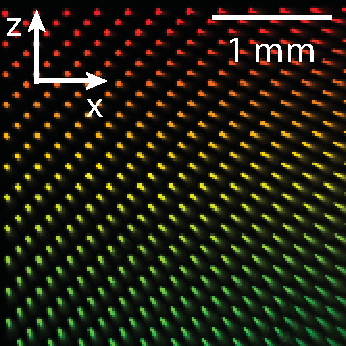
\includegraphics[width=0.15\textwidth]{./figures/figure15}
%  \caption{%Maximal intensity image of an image sequence of laser scanning positions measured for a Nikon A1 scan lens, where colour represents each recorded image for a sampled subset.
%  Illumination profile in the $xz$ plane for 400 scan positions, as measured through a Nikon A1 scan lens.
%  }
%  \label{fig:15}
%\end{figure}

\subsection{Scan lens characterisation}

To accurately measure the deviation solely caused by the scanning system, a camera (Thorlabs DCC1545M) was mounted directly after the scan lens and an attenuated beam was imaged directly onto the sensor.
The full range of the scanning unit was considered by incrementing mirror control voltages ($V_x$, $V_z$) linearly in input space.
%through discrete $xz$ postions%mirror voltages
and imaging the illumination beam in $xz$ for each step,
%capturing an image of the beam for each
as shown in Figure \ref{fig:2}a.
Each beam profile was fit with a 2D Gaussian to create a map of $xz$ illumination positions corresponding to constant steps in scan lens.
%voltage to position calibration map.
Figure \ref{fig:2}b and \ref{fig:2}c show the residual deviation from desired positions when using a 4~pt and 3~pt registration respectively.
The 4~pt correction is more faithful to experimental values.
%Figure \ref{fig:2}c computes the average discrepancy incrementing through the observation volume, using more of the area of the scan lens and the regions where the scan lens' telecentricty breaks down.
The figure verifies that a 4~pt correction %will always
produce a more valid fitting for a beam scanned across a telecentric lens, with a more significant improvement becoming apparent when using a larger region of the scan lens.

\begin{figure}
  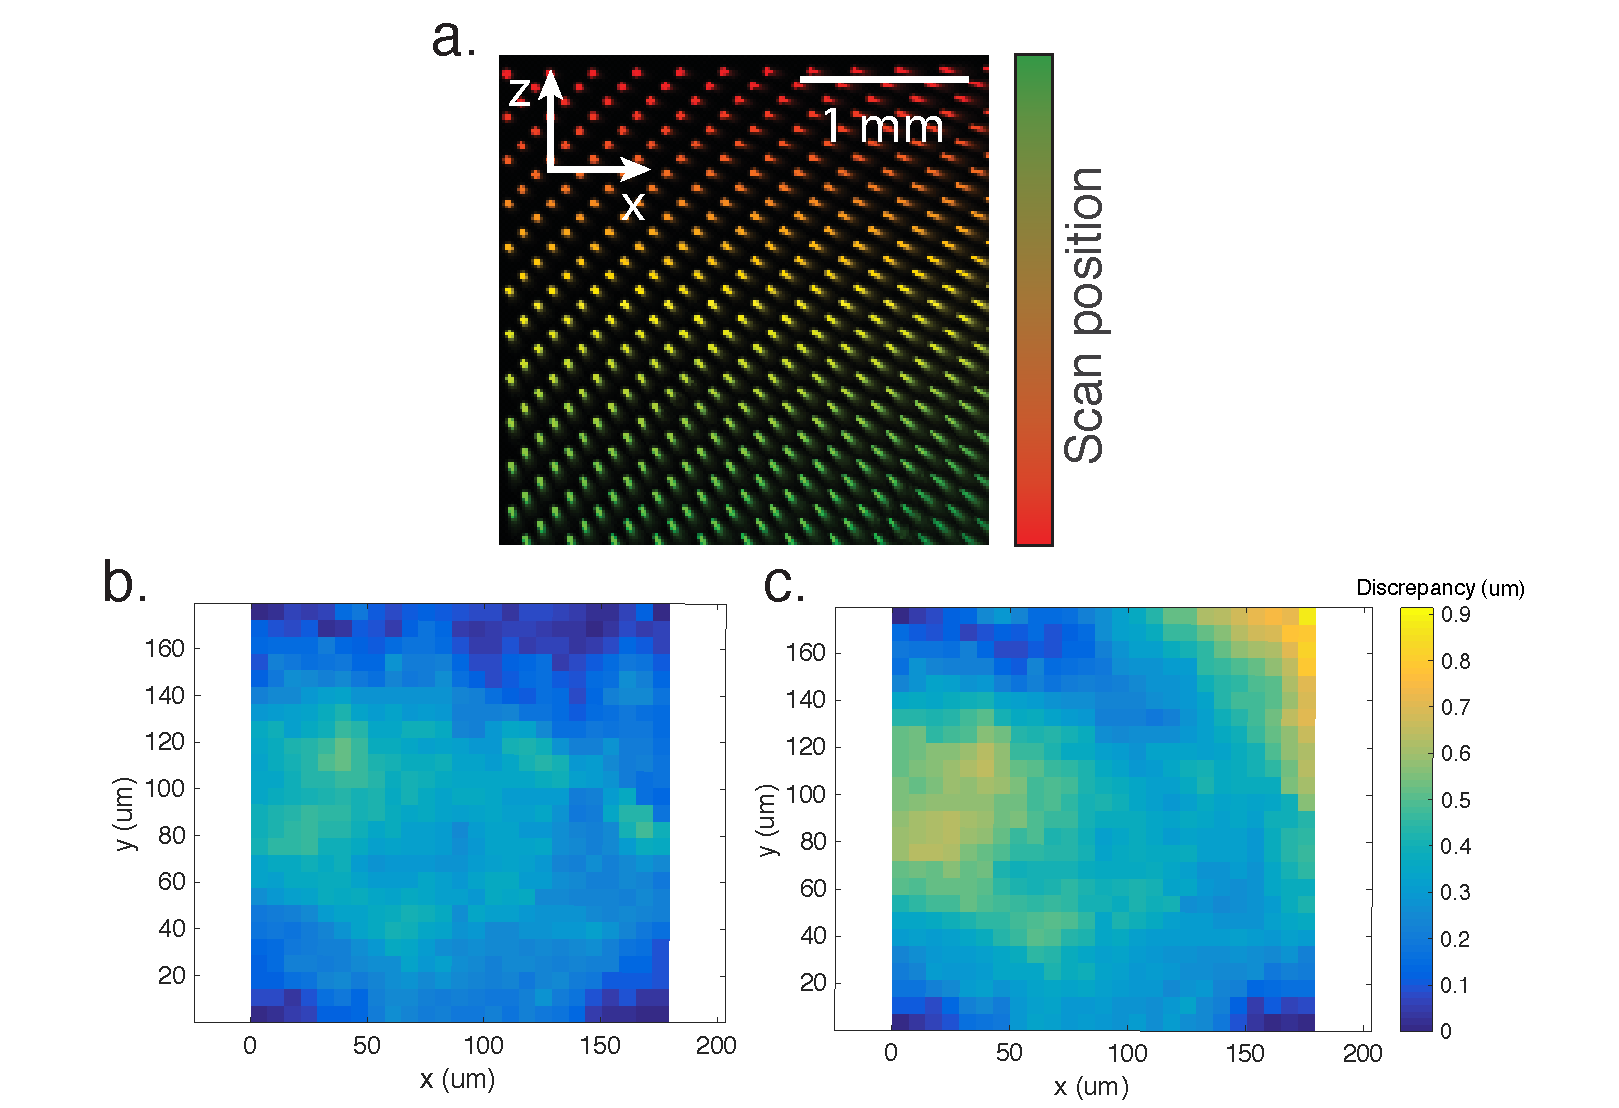
\includegraphics[width=\columnwidth]{figure2}
  \caption{\textbf{Scan lens characterisation} | Figure (a) shows the Illumination profile in the $xz$ plane for 400 scan positions, %as measured through a Nikon A1 scan lens.
  with a 3~pt registration.
  The beam positions in %the images from the stack in Figure
  (a) were each localised by fitting a 2D Gaussian.
  The identified positions %fit
  using a 3~pt (c) and 4~pt (b) %fitting over a quarter of the scan lens
  %(b) and (c) then each show
  show that the positional discrepancy of the 3~pt method is largely fixed by the 4~pt registration.
  %the positional discrepancy from ground truth data using their respective corrections.
  % (c) increments the windows in (a) and (b) to retrieve an average correction discrepancy as a function of distance from the centre of the scan lens, measured in image space.
  %(c) shows a 3~pt correction progressively worsening.
  }
  \label{fig:2}
\end{figure}

\subsection{\emph{in situ} characterisation}

In real samples for
light-sheet microscopy, %the error introduced by the scanning unit contributes to
a mismatch between the detection plane and the illumination plane %, this causes out-of-focus fluorophores to dominate.
%which
can %greatly
reduce image fidelity due to decreased illumination in the imaging plane as well as
excess background fluorescence.
Figures \ref{fig:3} show the 4~pt registration largely eliminates this %with the
mismatch for real samples including fluorescent beads, dyes and a model organism.
%; higher order corrections provide diminishing returns.
%TODO fix this
%The 4~pt correction intends to better align the detection and focal planes for each image, as such a 3~pt correction will produce a non-uniform blurring in comparison.

\begin{figure*}[h]
  \includegraphics[width=\textwidth]{figure32}
  \caption{\textbf{\emph{in situ} characterisation} |
  (a-b) Ratios of intensity maxima of localised fluorescent bead images
  %Localised beads' peak intensities
  were compared in 3D observation volumes %recorded
  using 3 and 4~pt corrections.
  (a) These ratios show an %peak
  average 42\% increase in contrast for the 4 pt. case, %peak intensity
  with an increasing effect when traveling axially (b).
  (c) The corresponding graph for a beam scanned through dye solution also demonstrates greater light capture efficiency which becomes more significant with depth.
  The image maxima was taken as a good measure of beam to image plane focus.
  In (d) we show a transgenic Zebrafish expressing mCherry:beta-actinCAAX, in which the membrane contrast is substantially improved by the 4~pt registration.% and is used to visually compare the 4~pt and the 3~pt correction.}
  }
  \label{fig:3}
\end{figure*}

%To demonstrate %validate
%the 4~pt correction, f
In Figure \ref{fig:3} a-b Fluorescent beads (TetraSpeck 100nm Microspheres) were dispersed in 1.5\% agarose at 1:1000 concentration and imaged using a 3~pt and a 4~pt registration.
Each bead (of $\sim$500) was localised in 3D %laterally localised manually in a maximal intensity projection %, with the assumption that the beads were sufficiently sparse to not overlap.
%and axially using maximum peak image variance.
%Once localised, each bead's peak
and its peak fluorescence intensity was compared in the 4~pt and 3~pt case, and was found to be, on average,
%The intensity improvement in the 4~pt case's distributed peak average was
42\% higher across the entire volume ($512~\si{\micro\metre} \times 512~\si{\micro\metre}\times 100~\si{\micro\metre}) $ for the 4~pt registration.
For a 10~\si{\micro\metre} light-sheet this corresponds to an axial light-sheet mismatch of 6.9~\si{\micro\metre} on average, for the 3~pt case. %TODO recalculate.
%Figure \ref{fig:3} reiterates the message from Figure \ref{fig:2} in that the deeper one penetrates the sample the more valid and useful a 4~pt correction is.
%We implmeneted this in our iSPIM.
%We imaged beads coventionally and with slit scanning then with this new tntechnique and with slit scanning
%\subsection{Results and discussion}
%discuss results
 %Here are images with and with 4~pt correction and 3~pt correction
 %Here is a graph of me drifting the laser profile into the non-telecentric region of the lens:
	 %Non-telecentricity is now more corrected for compared to the old calibration technique
The experiment from Figure \ref{fig:2} was repeated in the light-sheet microscope using dye solution for Figure \ref{fig:3}c.
The scanning beam was paused and iterated again through discrete positions in the imaging volume.
Each record fluorescent dye image was characterised by a focus measure, obtained by finding the intensity maximum through the focus of the light-sheet for each beam position.
As expected, greater depth degraded how well matched the beam was to the focal plane more sharply for the 3~pt correction than the 4~pt.

The advantages of using a 4~pt correction were then finally demonstrated in Zebrafish (\emph{Danio rerio}), a model organism  ubiquitous in light-sheet imaging.
The sample used in Figure \ref{fig:3}d was transgenically expressing mCherry near the cellular membrane (Beta-actin: mcherryCAAX) and mounted in 1.2~\% agarose;
the sample itself was 4 hours post-fertilisation.

\section{Conclusions}

Considerations in registration between detection and illumination volumes\cite{royer_adaptive_2016} are becoming increasingly pertinent with the current trends of exceptionally large samples\cite{chen_expansion_2015} being imaged at diffraction limited resolution and at depth\cite{wang_direct_2015,truong_deep_2011}.
Advances in cameras\cite{zheng_0.5_2014,brady_multiscale_2012}, optics\cite{sofroniew_large_2016} and fast piezo technology will further exaggerate errors introduced when using linearly generated waveforms in the next generation of light-sheet microscope.

We have demonstrated that, for iSPIM systems using virtual light-sheets, a 4~pt correction (non-linear waveform generation) versus a 3~pt correction (affine waveform generation) will better counteract errors introduced by beam scanning optics, conveniently and for minimal computational cost.
%TODO 5pt or further.
%When compared in bead samples, the 4~pt correction presented a 42\% improvement of captured light intensity over the 3~pt correction for a volume of $512\times512\times100 \si{\micro\metre}^3$.
%The homographic correction presented here attempts to utilise all available degrees of freedom at no extra loss, however it should be noted that systems with more degrees of freedom\cite{royer_adaptive_2016} (additional mirrors) produce a similar effect for further cost and complexity.
%The 4~pt correction was computed using matrix operations which %helped minimise computation time for
%facilitated dynamic re-generation of waveforms.


%The homographic correction presented here attempts to utilise all available degrees of freedom at no extra loss, however it should be noted that systems with more degrees of freedom\cite{royer_adaptive_2016} (additional mirrors) produce a similar effect for further cost and complexity.


%The technique acts to maximise
%When only a small area of the scan lens is used the two corrections tend to converge.


% Boyden~\emph{et~al} are currently expanding fixed samples to 4.5x their size with a view to increasing that to 20x;
% 2P light-sheets have reached 700\si{\micro\metre})using adaptive optics;
% Physique Instrument (PI) are now producing nanometer precision piezo objective travelers with a range of 2mm;
% gigapixel cameras may soon be commercially viable \cite{zheng_0.5_2014,brady_multiscale_2012}
% and large field of view \emph{meso}lenses are showing promise \cite{sofroniew_large_2016}.


%It should be noted that such a correction is needed less in systems which are more robust to optical field-curvature, for instance top-end confocal
%scanning units typically use four individual mirrors, with each pair being used to create an effective telecentricity without the need for lenses except for relay optics.
 %This is really good, can be used lalallala
 %Could be applied to other volumetric imaging technqiues using as confocal and image scanning. . . . .
 %Would be more pronounced in high NA.
